\documentclass[12pt]{report}
\usepackage{tkz-graph}
\usetikzlibrary{positioning}

\SetGraphUnit{4}
\GraphInit[vstyle=Simple]
\SetVertexSimple[MinSize=20pt, LineColor=blue!20, FillColor=blue!20]
\tikzset{main node/.style={circle, fill=blue!15, draw, minimum size=1cm, inner sep=0pt}}

\begin{document}

	\begin{center}
		\section*{TikZ Graphs}
	\end{center}
	
	\begin{enumerate}
		\item The \texttt{tkz-graph} package is used.
		\item The styling of each node is set using \texttt{\textbackslash tikzset}
		\item To change the position of nodes, you can define the positioning using adverbs \texttt{below right = 1.5cm and 1.5cm of A}
	\end{enumerate}

	\begin{center}
		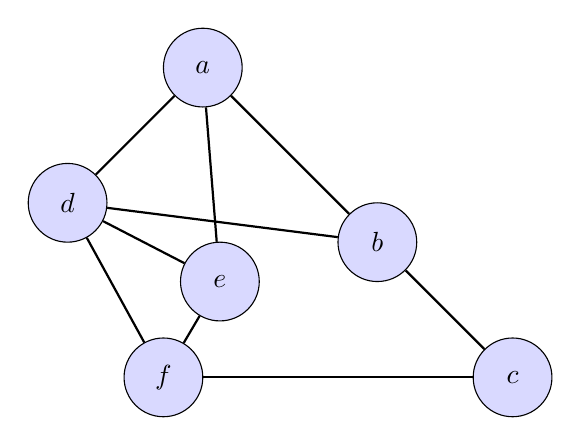
\begin{tikzpicture}
			% Define each node
			% The value between parenthesis is the name of the node
			% The name of the node can be used to draw edges, and position other nodes
		    \node[main node] (A) {$a$};
		    \node[main node] (B) [below right = 1.5cm and 1.5cm of A]  {$b$};
		    \node[main node] (C) [below right = 1cm and 1cm of B] {$c$};
		    \node[main node] (D) [below left = 1cm and 1cm of A] {$d$};
		    \node[main node] (E) [above left = 0.5cm and 3cm of C] {$e$};
		    \node[main node] (F) [below left = 1cm and 2cm of B] {$f$};
		
		    \path[draw, thick]
		    % Draw edges between nodes
		    (A) edge node {} (B)
		    (A) edge node {} (D)
		    (A) edge node {} (E)
		    % Include text on edge by adding text inside {}
		    (B) edge node {} (C)
		    (B) edge node {} (D)
		    (C) edge node {} (F)
		    (D) edge node {} (E)
		    (D) edge node {} (F)
		    (E) edge node {} (F);
		\end{tikzpicture}
	\end{center}
	
\end{document}